\paragraph{The bug class.}
An HTTP/1.1 server that receives a request body via chunked
transfer encoding must, somewhere on the data path, transition
decoded body bytes from the wire-level parser into application
code. The specification~\cite{rfc9112} fixes the wire format
(\texttt{<hex-size>\textbackslash r\textbackslash n<bytes>\textbackslash r\textbackslash n},
terminated by a zero-length chunk) but is silent on how a parser
should schedule callbacks into the application: per chunk, per
\texttt{recv()} batch, per fixed-byte threshold, or fully buffered.

We measure which of those choices each production HTTP server has
adopted as the default, and the cost in single-core CPU of the
chosen granularity under a pathological-but-RFC-compliant input
shape: an $N$-byte body encoded as $N$ one-byte chunked-TE chunks.

\paragraph{Headline finding.}
Of 27 production HTTP servers measured across 7 language ecosystems
plus three C servers:

\begin{itemize}
\item \textbf{1 server}, Kestrel on ASP.NET Core, moves the per-chunk
  cost off the async/await scheduling boundary via
  \fname{System.IO.Pipelines}. Kestrel still pays a per-chunk
  parsing cost (\SI{3.6}{\micro\second}/chunk steady-state) but
  the resulting end-to-end cost is dominated by the synchronous
  parser loop rather than a per-chunk task switch.
\item \textbf{22 servers} are linear-but-per-chunk vulnerable, with
  per-chunk costs spanning a factor of \(\sim 50\times\) (\SI{2.1}{\micro\second}/chunk
  for uvicorn+httptools, \SI{114}{\micro\second}/chunk for nginx as
  origin).
\item \textbf{4 servers} exhibit superlinear scaling consistent
  with an asymptotic \(\Theta(N^2)\) mechanism observed in the
  profile, with measured exponents in the 1.0--2.0 range over our
  $N$ range: Node's built-in \fwid{http.Server}, \fwid{express},
  \fwid{fastify}, and Elixir's \fwid{bandit}. The Node trio reaches
  measured exponent $\sim 1.7$--$2.0$ in our $N$ range; bandit's
  measured exponent of $\sim 1.0$--$1.3$ over the same range is
  bounded by the iolist-size walk profile and extrapolates
  asymptotically to $\Theta(N^2)$.
\end{itemize}

\noindent
Figure~\ref{fig:headline-uschunk} ranks all 27 by per-chunk cost
under the canonical Mode B probe (paced \SI{100}{\micro\second}
gap, \(N{=}\num{250000}\), 1 vCPU container).

\paragraph{Contributions.}
\begin{enumerate}
  \item The first systematic cross-ecosystem measurement of
  chunked-TE delivery granularity in production HTTP servers,
  spanning 7 language ecosystems and three C servers
  (Section~\ref{sec:perframework}, Section~\ref{sec:synthesis}).
  \item Identification of two distinct routes to superlinear
  scaling, one previously characterized as an availability issue
  (Node's Readable substrate) and one not (\fwid{bandit}'s
  iolist accumulator).
  \item Identification of a single existence-proof
  (\fname{System.IO.Pipelines}/Kestrel) that the bug class can be
  structurally closed at the server layer; the design is not
  novel to this work but its security relevance has not been
  publicly named.
  \item A characterization of the "deploy behind nginx" mitigation:
  default nginx \emph{does} aggregate chunks for the upstream
  (Section~\ref{sec:mitigation}), but \fwid{HAProxy} does not.
  \item A mitigation taxonomy comparing server-side aggregation,
  application-side chunk limits (such as hyper's
  \fname{BodyExt::limit\_chunks(N)}~\cite{hyper_4008}), frontend
  buffering, and transport-layer rate limiting.
  \item A reproducer harness (per-server Dockerfile + standardized
  probe + JSON results, schema-validated) published with the paper.
\end{enumerate}

\paragraph{Roadmap.}
Section~\ref{sec:background} provides background on the chunked
encoding and on the dispatcher architectures we measure.
Section~\ref{sec:methodology} describes the measurement protocol.
Section~\ref{sec:perframework} treats each server individually.
Section~\ref{sec:synthesis} compares them.
Sections~\ref{sec:rootcause}--\ref{sec:mitigation} analyze root
cause, threat model, and mitigations.

\begin{figure}[t]
  \centering
  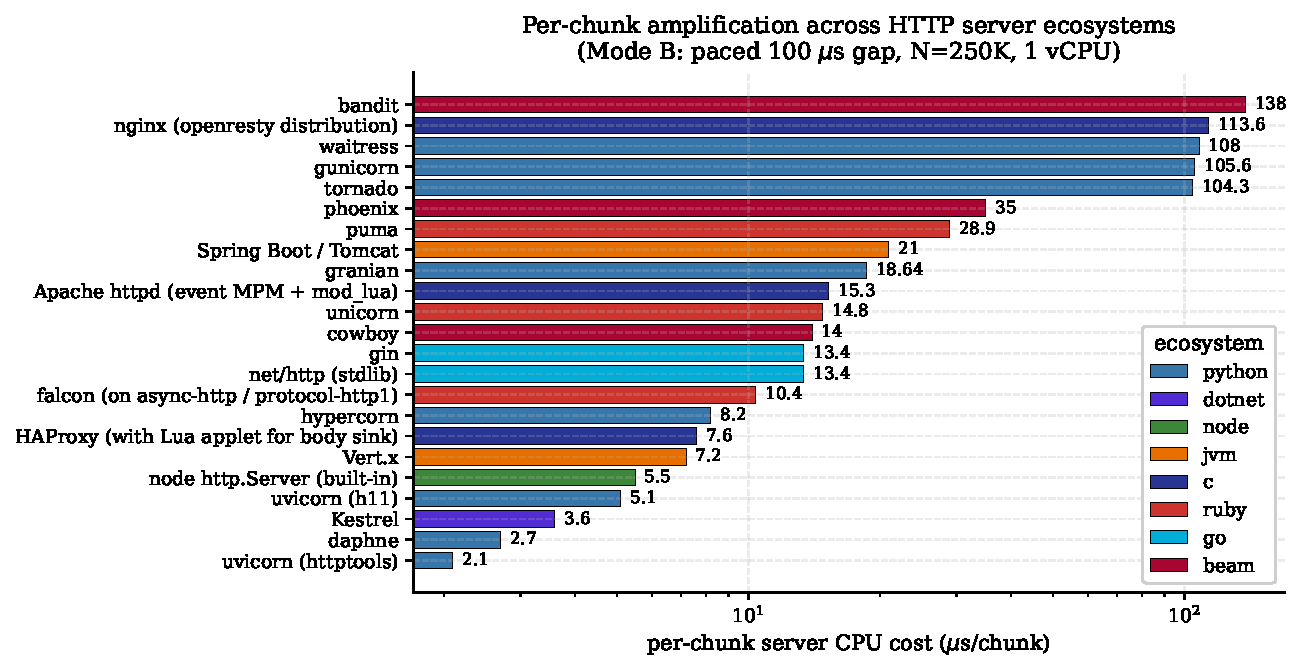
\includegraphics[width=0.95\linewidth]{figures/us_per_chunk.pdf}
  \caption{Per-chunk server CPU cost across all 27 servers measured
  (Mode B: paced \SI{100}{\micro\second} gap, $N{=}\num{250000}$
  one-byte chunks, 1\,vCPU container). Log-scale x-axis.
  Spans nearly three orders of magnitude. Kestrel
  (\textsc{BATCHES-CORRECTLY}, leftmost) is the single existence
  proof in our sample.}
  \label{fig:headline-uschunk}
\end{figure}

\begin{figure}[t]
  \centering
  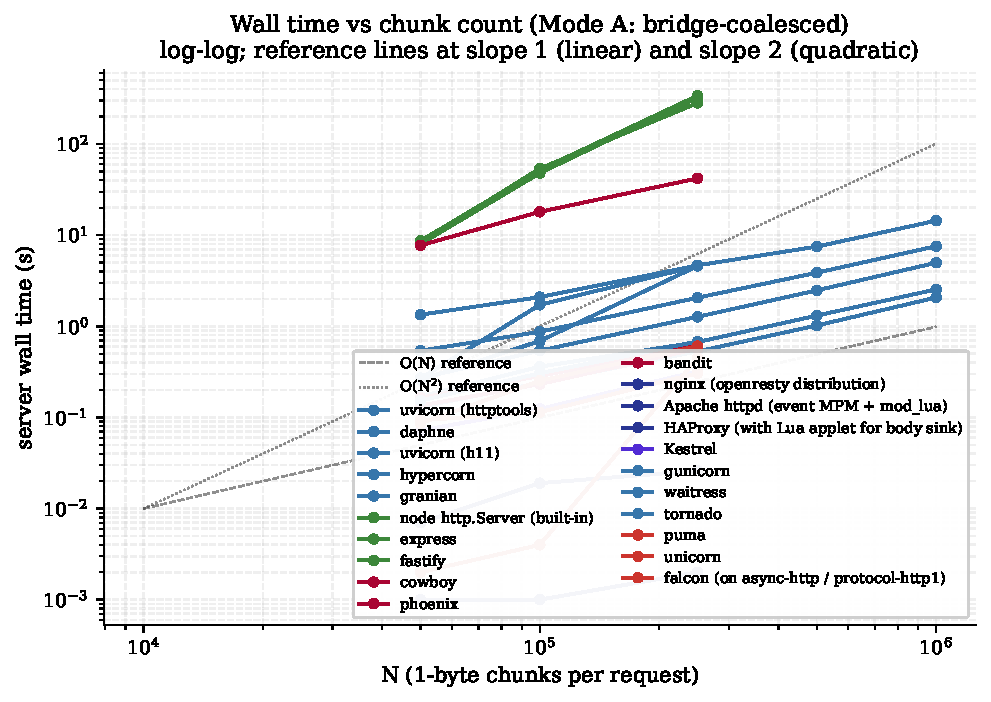
\includegraphics[width=0.95\linewidth]{figures/scaling_loglog.pdf}
  \caption{Wall time vs chunk count $N$ under Mode A
  (bridge-coalesced). Log-log axes; reference slopes at 1 (linear)
  and 2 (quadratic). The Node trio and \fwid{bandit} are the four
  data series that approach the quadratic reference.}
  \label{fig:scaling}
\end{figure}
